\documentclass[12pt, openany]{book}

% This is all the packages and settings and so on.
% It is using custom fonts that needs to be installed on the computer. If they are not present, they have to be added manually.
\usepackage[
	citestyle=ieee,
    bibstyle=ieee,
    style=numeric-comp,
    sorting=nty,
    maxbibnames=99, % Make sure we are printing all authors in the appendix
    ]{biblatex}

% Makes the last name first in the bibliography.
% \DeclareNameAlias{author}{last-first}
\DeclareNameAlias{author}{family-given}

% Specify the margins. This is 6.25inches in text with which
% can be used to size figures to the correct size.
\usepackage[a4paper, margin=2.5625cm]{geometry}

\usepackage{eso-pic}					% Packages for layout and graphics
\usepackage{graphicx}
\usepackage{tikz}
\usetikzlibrary{fadings}
\usepackage{setspace}
% \usepackage{tocloft}		 			% Fixing a bug with page style changes for toc
% \tocloftpagestyle{plain}
\usepackage{etoc} 						% Separate tocs for appendix and the rest
\usepackage{chngcntr}					% Count figures within chapters
\usepackage{booktabs}					% Table formatting
\usepackage{fancyhdr}					% Setting the style for header and footer.
\usepackage{tabularx}
\usepackage{multirow}                   % For better tables
\usepackage[hidelinks]{hyperref}		% Clickable links
\usepackage{nameref}					% References with names
\usepackage[parfill]{parskip}			% New line instead of indent for sections
\usepackage{tcolorbox}					% Create boxes around content
\tcbset{colback=white,arc=0mm}

\usepackage{amsmath}
\usepackage{mathdots}
\usepackage{yhmath}
\usepackage{siunitx}
\usepackage{array}
\usepackage{gensymb}
\usepackage{amssymb}
\usepackage{mathtools}              % Add text to math arrows.

\usepackage{cancel}
\usepackage{color}
\usepackage{multirow}
\usepackage{textcomp}               % Fixing warning for gensyb \perthousand
\usepackage{svg}                    % including svg files
\usepackage{caption}                % For subfigures
\usepackage{subcaption}
\usepackage{fontspec}
\usepackage{sectsty}
\usepackage{tocloft}

\usepackage[printonlyused]{acronym}


\counterwithin{figure}{section}
\counterwithin{table}{section}

% Specifying fonts
% \setmainfont{Georgia} 
% \setsansfont{Arial}
% \newfontfamily\footerfont{Georgia}

\chapterfont{\sffamily\fontsize{17}{17}}
\sectionfont{\sffamily\fontsize{14}{15}}
\subsectionfont{\sffamily\fontsize{13}{15}}
\subsubsectionfont{\sffamily\fontsize{12}{15}}

% Remove the title and make sure that the text is adjusted
% \usepackage{abstract}
% \setlength{\absleftindent}{0mm}
% \renewcommand{\abstractname}{\vspace{-\baselineskip}}
% \renewcommand{\abstractnamefont}{\sffamily\fontsize{14}{15}}
% \renewcommand{\abstracttextfont}{\normalfont\fontsize{12}{13}}

% Renaming and setting style of table of contents
\renewcommand*\contentsname{Contents}
\renewcommand*\cfttoctitlefont{\fontsize{16}{0}\bf\sffamily}
\renewcommand\cftchapfont{\fontsize{14}{0}\bf\sffamily}
\renewcommand\cftchappagefont{\fontsize{13}{0}\bf\sffamily}
\renewcommand\cftsecfont{\fontsize{12}{0}\sffamily}
\renewcommand\cftsecpagefont{\fontsize{12}{0}\sffamily}
\renewcommand\cftsubsecfont{\fontsize{12}{0}\sffamily}
\renewcommand\cftsubsecpagefont{\fontsize{12}{0}\sffamily}

% Styling the header and footer
\fancyhf{}
\fancyhead{}
\fancyfoot{}
\fancyhead[L]{\fontsize{11}{10}\selectfont\leftmark}
\fancyfoot[R]{\footerfont\thepage}
\setlength{\headheight}{15.5pt}


\fancypagestyle{plain}{
    \fancyhf{}
    \fancyhead{}
    \fancyfoot{}
    \renewcommand{\headrulewidth}{0pt}
    \fancyfoot[R]{\footerfont\thepage}
}

\pagestyle{fancy}

% Making the command for placing text in random locations
\newcommand\PlaceText[3]{%
\begin{tikzpicture}[remember picture,overlay]
\node[outer sep=0pt,inner sep=0pt,anchor=south west]
  at ([xshift=#1,yshift=-#2]current page.north west) {#3};
\end{tikzpicture}%
}

% Disable hyphenation
\pretolerance=10000
\tolerance=2000
\emergencystretch=50pt


% Defining files for bibliography
%\addbibresource{ref.bib}
\addbibresource{references.bib}
% Add a second bibliography file for the second author to allow
% both to update it through the mendeley integration.
% \addbibresource{ref-author-2.bib}

% Defining document information
\title{Template}
\newcommand{\subtitle}{KTH Thesis Report}
\author{<Author Name and Author Name>}

\begin{document}
\setstretch{1.4}

% The front page of the document
\pagenumbering{roman}
\makeatletter
\begin{titlepage}

\vspace*{-4.6\baselineskip}
\hspace*{-0.15\textwidth}
\includegraphics[width=0.2\paperwidth]{setup/img/kth-logo.jpg}
\par\vspace*{2.5\baselineskip}

\PlaceText{65mm}{12mm}{\fontsize{12}{0}\sffamily DEGREE PROJECT IN TECHNOLOGY,}
\PlaceText{65mm}{17mm}{\fontsize{12}{0}\sffamily SECOND CYCLE, 30 CREDITS}
\PlaceText{65mm}{22mm}{\fontsize{12}{0}\sffamily\itshape STOCKHOLM, SWEDEN \the\year}

~\\

\makebox[0pt][l]{%
\begin{minipage}[b]{0.25\textwidth}
~\\
\end{minipage}
\begin{minipage}{0.65\textwidth}
\begin{flushleft}
{\fontsize{28}{24}\bf\sffamily\@title\\}
\vspace{1cm}
{\fontsize{19}{17}\bf\sffamily \subtitle\\}
\vspace{1cm} 
{\fontsize{16}{18}\sffamily \@author}\\
\end{flushleft}
\end{minipage}
}


% \hspace*{-3cm}\begin{minipage}[b]{63.5mm}
% ~\\
% \end{minipage}
% \begin{minipage}{0.65\textwidth}
% \begin{flushleft}
% {\fontsize{28}{24}\bf\sffamily\@title\\}
% \vspace{0.5cm}
% {\fontsize{19}{17}\bf\sffamily \subtitle\\}
% \vspace{0.5cm} 
% {\fontsize{16}{0}\sffamily \@author}\\
% \end{flushleft}
% \end{minipage}


\AddToShipoutPictureBG*{%]
    \AtPageLowerLeft{%
        
\includegraphics[width=1.0\paperwidth]{setup/img/kth-footer.png}
    }%
}

\PlaceText{70mm}{280mm}{\color{white}\fontsize{12}{0}\sffamily KTH ROYAL INSTITUTE OF TECHNOLOGY }
\PlaceText{70mm}{285mm}{\color{white}\fontsize{8}{0}\sffamily ELECTRICAL ENGINEERING AND COMPUTER SCIENCE }
\end{titlepage}
\makeatother

\newpage
% !TEX root=../../mt-motion-analysis.tex
% \newpage
% Anterior Cruciate Ligament (ACL)
\tableofcontents
\chapter*{Abstract}
\addcontentsline{toc}{chapter}{Abstract}
Injuries to the \gls{acl} are severe injuries, common among the physically active young to middle aged population. After suffering from such an injury, the patient typically face a lengthy rehabilitation process. Usually, it takes 1-2 years before an injured knee returns to pre-injury performance, if that is ever achieved. The risk of re-injury is high and is increased by early return to sports. One measure which has been suggested as an indicator of the increased risk of re-injury, and hence could work as an indicator of when to return to normal activity, is altered postural orientation. The postural orientation describes the positions of different body parts in relation to each other and the surroundings. Assessment of this is a time consuming task requiring human experts trained to finds such alterations. This thesis propose a method to automate this task by analyzing videos recorded with a regular video camera, e.g. a mobile phone.

The proposed method uses well established deep learning techniques, in this case HRNet with DARK-pose, to extract body part positions from each video frame. Deep learning based models are trained in a supervised fashion to classify the sequences of extracted keypoints. Models trained to perform according to different metrics were combined in ensembles classifying the quality of the postural orientation on an ordinal scale from 0 (Good), via 1 (Fair), to 2 (Poor).

We evaluated the method on four different segment-specific \glspl{poe} when the patient performed a single leg squat. The different POEs were trunk, pelvis, femoral valgus, and \gls{kmfp}. For femoral valgus and trunk a classification accuracy of 82.3\% and 80.0\%, respectively, was achieved. The corresponding number for \gls{kmfp} was 90.3\%, but this data was heavily imbalanced. The pelvis was the most difficult to analyze resulting in an accuracy of 73.3\%.

The most important contribution of this thesis is to provide a foundation and a number of insights of what is needed before introducing a method like this for clinical use.

\chapter*{Acknowledgements}
\addcontentsline{toc}{chapter}{Acknowledgements}
The computations were enabled by resources provided by the Swedish National Infrastructure for Computing (SNIC) at Chalmers Centre for Computational Science and Engineering (C3SE) partially funded by the Swedish Research Council through grant agreement no. 2018-05973.

Regarding thank yous I would like to begin by giving a big one to Eva Ageberg and Mark Creaby for your ideas and insights. Secondly I would like to thank Jenny Älmqvist Nae for introducing this field to me, for explaining concepts which were very alien to me six months ago, and for assessing so many videos. Finally I would like to give a big thank you to Andreas Jakobsson for your enthusiasm and ideas throughout the project, for finding so many missing commas in this text, and for being a source of inspiration.

% “And now here is my secret, a very simple secret: It is only with the heart that one can see rightly; what is essential is invisible to the eye.”
% ― Antoine de Saint-Exupéry, The Little Prince

\newpage
\etocdepthtag.toc{mtchapter}
\etocsettagdepth{mtchapter}{subsection}
\etocsettagdepth{mtappendix}{none}
\thispagestyle{plain}
% \setstretch{1}
\printglossary
% \setstretch{1}
% \listoffigures
% \listoftables



\pagenumbering{arabic}

% !TEX root=../../mt-motion-analysis.tex
\chapter{Introduction}



skriv om risker med bias fr dataset osv...

\section{Medical background}
skriv om acl och varf;r detta arbete beh;vs
related work, se ref i mendeley osv
\subsection{POEs}
...

\subsection{avgr'nsningar}
typ om att bara SLS analyseras? och lite s[nt.. kanske att 3d inte utv'rderas? eller att det utv'rderades litgrann??

% !TEX root=../../mt-motion-analysis.tex
\chapter{Background - Deep learning}

% \section{Machine learning - ELLER BARA DL??} \label{sec:ML}
A supervised machine learning problem can be described as finding a mapping between some input and output data, e.g. an image and a category, based on labeled input-output combinations. The idea with such methods is that a mapping found for the available data also should represent unseen data of the same type, i.e. it should generalize. To be able to get a measure of this generalization the available data is commonly divided into two parts, training data and test data. The training data is used to find the mapping and the test data is used to evaluate how well it performs on unseen data \cite{Bishop2006}.

This chapter gives a brief introduction to a special type of machine learning called deep learning, which forms the basis of this work.

FIXAA DEN HAR SECTION INDELNINGEN...
\section{Deep Neural Networks}
\glspl{dnn} are combinations of linear and non-linear functions trained to approximate some other, potentially very complicated, function. The output of the network is formed as $f(x) = f_n \circ f_{n-1} \circ \hdots \circ f_1 \circ f_0(x)$ resulting in the layer terminology since the output from one function is passed as input to the subsequent one \cite{Goodfellow2016}.

Below the layers functions used in our work are briefly explained.

\subsubsection{Dense layer}
The dense, or fully connected, layer is the basic model for a feedforward network. The outputs of such a layer is formed as linear combinations of the inputs and bias terms. Usually a non-linear activation function is applied to to this to be able to capture more general behaviors, resulting in the output

\begin{equation}
 y_i = h\Big( \sum_{j=1}^D w_{ij}x_j + b_i \Big).
 \label{eq:dense}
\end{equation}

$h(\cdot)$ is a, possibly non-linear, activation function. $x_j$, $j \in \{1, \hdots, D\}$ are the inputs to the layer, $w_{ij}$ and $b_i$ are the weights and biases learned during training \cite{Bishop2006}. A network with two dense layers is shown in Figure \ref{fig:dense}.

\begin{figure}
 \centering
 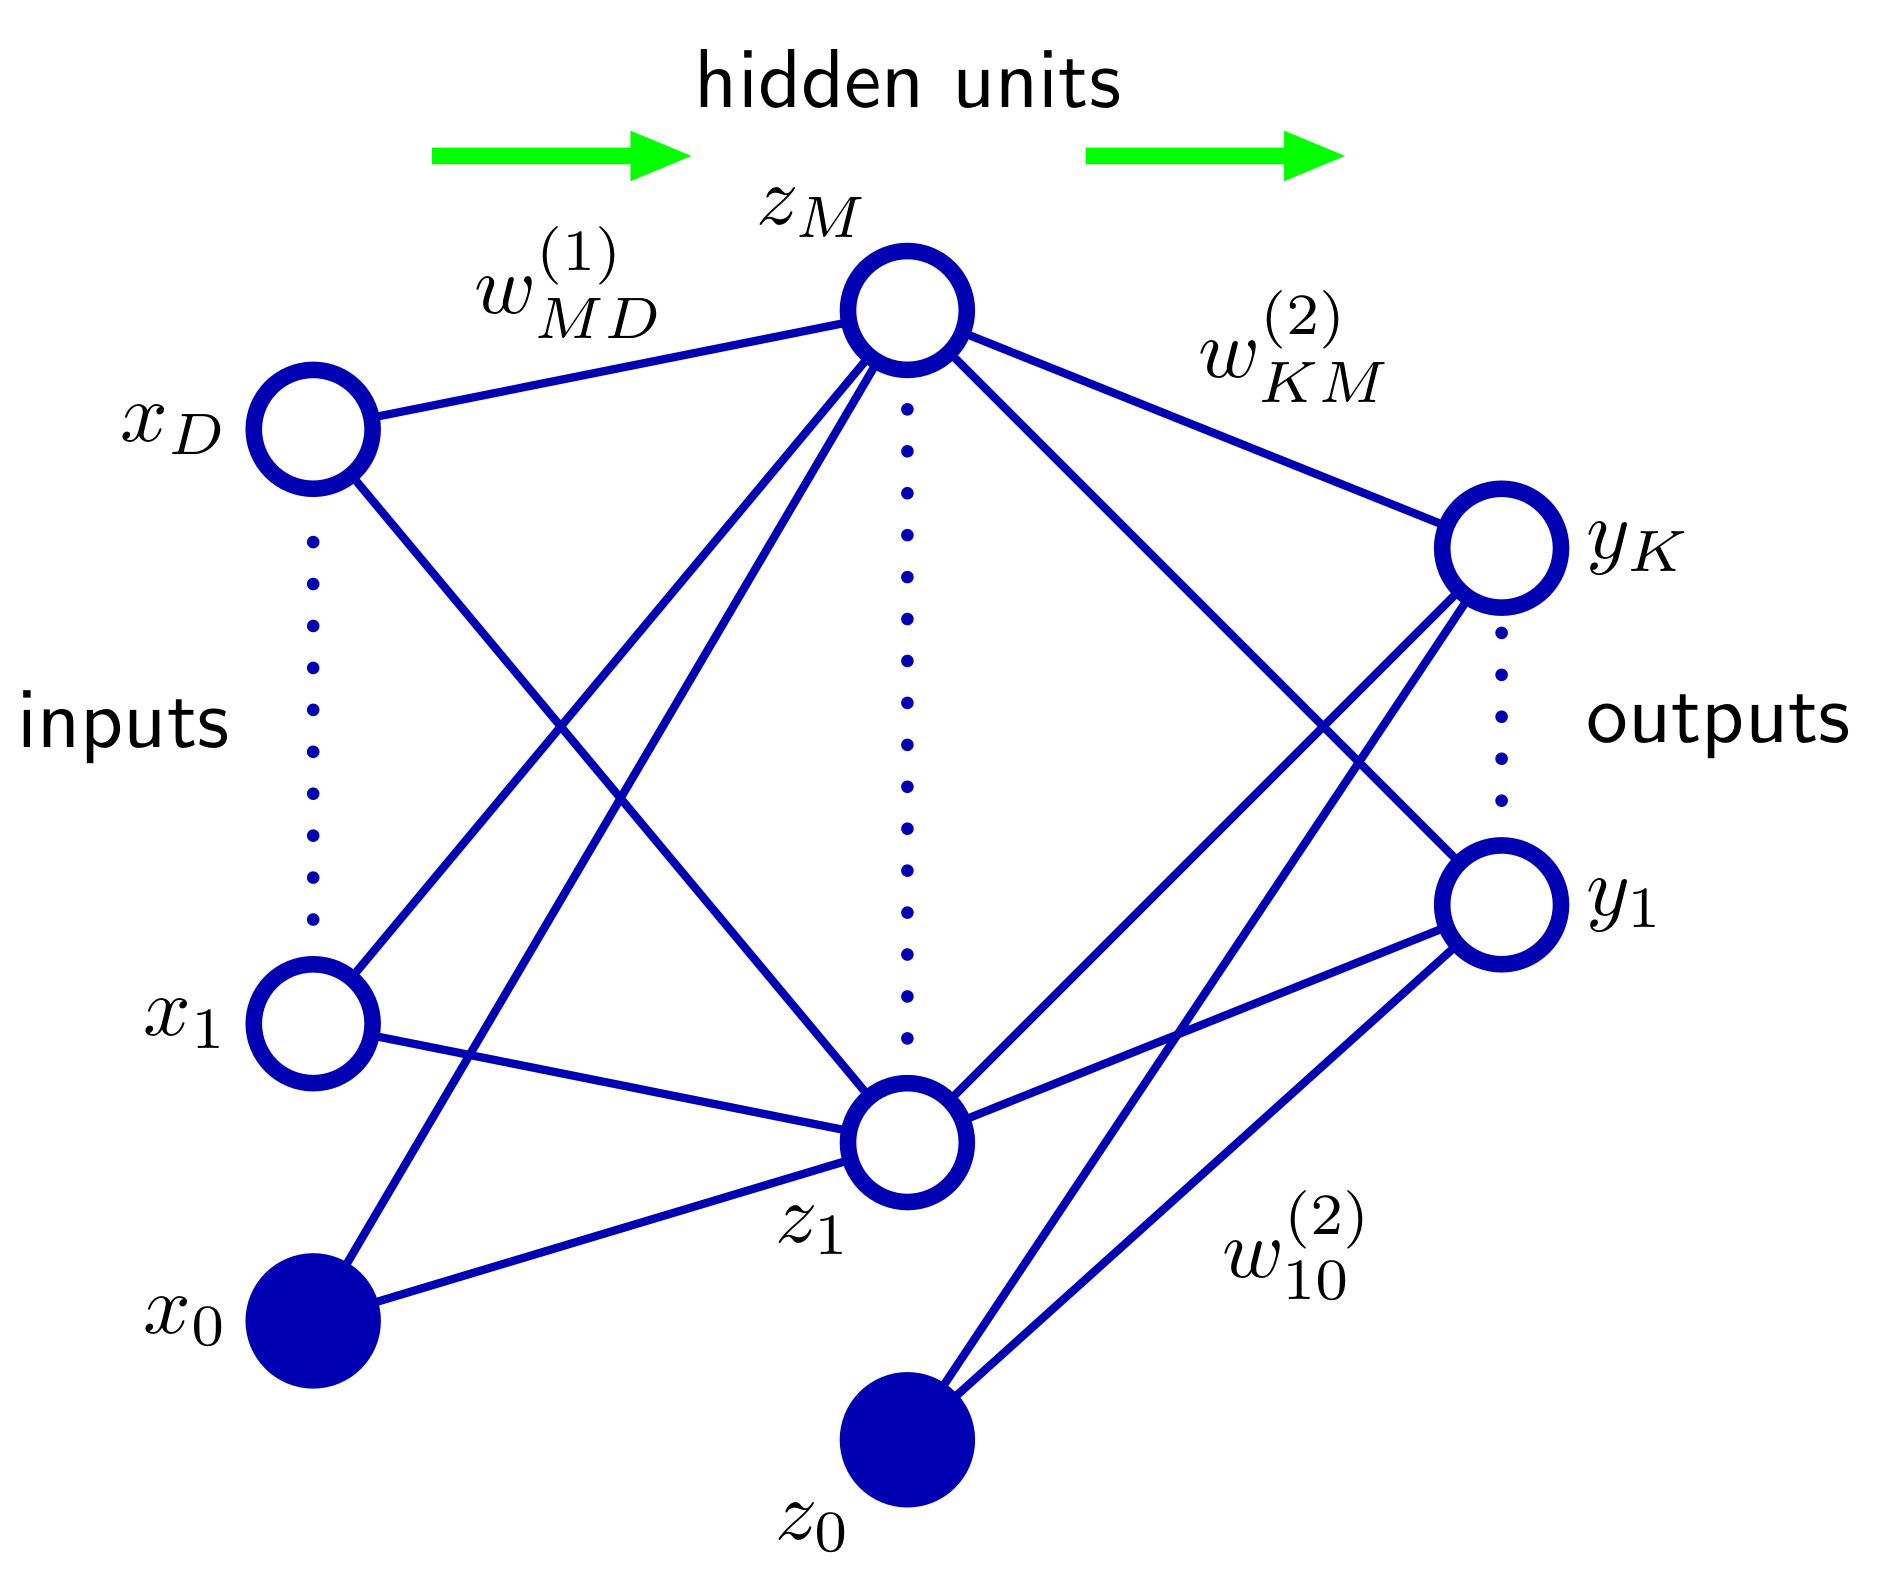
\includegraphics[width=0.5\textwidth]{files/figs/mlp.png}
 \caption{Feedforward neural network with two densely connected layers. Each line corresponds to one trainable parameter. $x_0$ and $z_0$ can be seen as ones added to the inputs introducing the bias terms \cite{Bishop2006}.}
 \label{fig:dense}
\end{figure}

\subsubsection{Convolutional layers}
Convolutional layers have proved successful for feature extraction from for instance time series or images. A reason for this is that they are equivariant to translation, meaning that patterns in a time series will be recognized in the same way no matter at which time steps they occur. The 1D convolution operation can be seen in \eqref{eq:conv}. When applied to for instance images it is performed in two dimensions.

\begin{equation}
 (x * w)(t) = \sum_{a=-\infty}^\infty x(a)w(t-a)
 \label{eq:conv}
\end{equation}

$x$ is the input and $w$ is the kernel or filter which consist of the trainable parameters. As the kernel size is not affected by the input size the convolutional layer can be applied to inputs of different size, which is not possible with for instance the fully connected layer \cite{Goodfellow2016}.

, layers, optimizers

\section{Training of }
% The training of a network is performed by evaluating a loss function, which describes the desired behavior, on the training data.

During training of a network a loss function, $\mathcal{L}$, which describes the desired behavior, is evaluated on the training data. To improve the performance of the model its parameters are changed to minimize this loss. In deep learning problems this optimization is usually performed with some gradient descent inspired method, shown in \eqref{eq:grad-desc}, where the parameters are updated in the direction which reduces the loss the most. With a large training data set the computation of the gradient quickly becomes expensive. A remedy for this has been to use stochastic or mini-batch gradient descent methods. Such algorithms use one or a few data points from the training set to estimate the gradient for each parameter update. Algorithms common today often use momentum, where previous gradients affect the parameter update direction, and adaptive learning rates (step size of parameter update), allowing different learning rate for different parameters \cite{Goodfellow2016}. One example of such a method is the Adam optimizer \cite{Kingma2015}.

\begin{equation}
 \pmb{W}_{k+1} = \pmb{W}_k - \alpha \pmb{D}
 \label{eq:grad-desc}
\end{equation}
\begin{conditions}
 $$\pmb{W}_k$$     & = & model parameters at iteration $k$ \\
 $$\alpha$$        & = & learning rate or step size \\
 $$\pmb{D}$$       & = & parameter update direction, e.g. $\frac{\partial \mathcal{L}}{\partial \pmb{W}}$ or a weighted average of earlier gradients
\end{conditions}

The gradients of the loss with respect to the model parameters are calculated using the back-propagation algorithm \cite{Rumelhart1987} which recursively uses the chain rule, \eqref{eq:chain}, to propagate the loss gradient through the network.

\begin{equation}
 \frac{dz}{dx} = \frac{dz}{dy}\frac{dy}{dx}
 \label{eq:chain}
\end{equation}

For a network where $f_0, f_1, \hdots, f_n$ denotes the outputs of the $n+1$ layers, with corresponding layer parameters $\pmb{w}_0, \pmb{w}_1, \hdots, \pmb{w}_n$ and loss function $\mathcal{L}$ the gradient is calculated by first performing a forward pass of input $\pmb{x}$. This allows for computation of the the gradient w.r.t. the output of the final layer, $f_n$, either analytically or using automatic differentiation. As both the structure and the parameters of the layers are known this can be used to calculate the gradient w.r.t. the parameters in that layer, $\pmb{w}_n$, as well as the output of the previous layer, $f_{n-1}$. By applying \eqref{eq:bp-layer} recursively the gradient is propagated through the network and from this \eqref{eq:bp-params} gives the gradients needed for the optimization.

\begin{subequations} \label{eq:backprop}
 \begin{align}
  \frac{\partial \mathcal{L}}{\partial f_k} & = \frac{\partial \mathcal{L}}{\partial f_{k+1}} \frac{\partial f_{k+1}}{\partial f_k} \label{eq:bp-layer} \\
  \frac{\partial \mathcal{L}}{\partial \pmb{w}_k} & = \frac{\partial \mathcal{L}}{\partial f_{k}} \frac{\partial f_{k}}{\partial \pmb{w}_k}    \label{eq:bp-params}
 \end{align}
\end{subequations}

\subsubsection{Loss functions}
For a classification problem with $K$ mutually exclusive classes the categorical cross-entropy is commonly used. With this loss the labels are one-hot encoded meaning that each label is represented by $K$ binary variables, i.e. $y_i \in \mathbb{Z}_2^K$. Each variable represents a class and $y_i^{(k)} = 1$ for the $k$ corresponding to the class of the label and 0 otherwise. The final layer of the model has $K$ outputs with softmax activation. The loss to be minimized is shown in \eqref{eq:cat-cross-entr} \cite{Bishop2006}.

\begin{equation}
 \mathcal{L}(\pmb{x}, \pmb{W}) = - \sum_{i=1}^N \sum_{k=1}^K \lambda^{(k)} y_i^{(k)} \log \hat{y}_i^{(k)}(x_i, \pmb{W})
 \label{eq:cat-cross-entr}
\end{equation}
\begin{conditions}
    $$y_i^{(k)}$$       & = & the correct binary label of class $k$ for data point $i$ in the training set \\
    $$\hat{y}_i^{(k)}$$ & = & the corresponding prediction from the model \\
    $$\lambda^{(k)}$$   & = & weight for class $k$.
\end{conditions}

The categorical cross-entropy will aim to maximize the predicted probability for the correct class. However, incorrect probabilities have no direct effect on the loss. To be able to affect what kind of errors the model makes in its predictions a modification of this loss can be used. This modified loss, here referred to as confusion-entropy, introduces a matrix, $U$, which can be seen as a target confusion matrix distribution. Entries in $U$ rewards predictions at the corresponding positions in the confusion matrix, including possible incorrect classifications.

skriv ekvation

skriv om att de har samma extrempunkt (ynk=1)



\subsubsection{activations osv, typ softmax, relu}



%The convolution, $(x * w)(t)$, can be seen as a weighted average of some points around $x(t)$

\section{Historical background of deep learning} \label{sec:dl-history}
In 1943 McCulloch and Pitts \cite{McCulloch1943} presented a mathematical model of a neuron which at the time had limited capabilities (e.g. it did not learn), but lay the foundations for much of what today is considered to be deep learning. Ivakhnenko and Lapa \cite{Ivakhnenko1965} introduced what would later be called deep learning with the first multi-layered network in 1965. The first convolutional network was introduced by Fukushima in 1980 \cite{Fukushima1980}. A few years later, in 1989, LeCun et al. \cite{LeCun1989} showed it possible to train such networks with backpropagation and illustrated their effectiveness for computer vision problems. In 2009 Raina et al. \cite{Raina2009} suggested that \glspl{dnn} could efficiently be trained on \glspl{gpu}. Krizhevsky et al. \cite{Krizhevsky2012} used this when they with AlexNet proved it possible to train deeper networks which also greatly outperformed models of the time at computer vision tasks. Since then deep learning based methods has been adopted in various fields, such as computer vision, natural language processing, and even autonomous vehicles \cite{NazmusSaadat2020}.

\section{Explainability} \label{sec:explainability}
Much of the recent progress in the deep learning space is inherently incomprehensible for us humans, due to its black-box nature and the size of the models \cite{Du2018}. However, explainability is important at many stages of the development of an AI-system. When the systems performance is at sub-human levels it simplifies for human experts to improve it. When the system achieves similar results human experts it can help enforce trust to the system. Finally, in a scenario where the AI outperforms humans it can help us get a better understanding of the problem \cite{Selvaraju2016}. With these methods playing a bigger role in fields such as healthcare the importance of explainable decisions also grows from a legal and ethical perspective \cite{Amann2020}.

\subsubsection{Gradient-weighted Class Activation Mapping (Grad-CAM)} \label{sec:grad-cam}
Although most deep learning models are not interpretable there are post-hoc methods which tries to explain decisions. Selvaraju et al. \cite{Selvaraju2016} suggested one such method, called \gls{grad-cam}, where an activation map is calculated which shows what parts of the data is important for the decisions. Considering a neural network with convolutional layers as feature extractors followed by \gls{gap} and dense layers for classification \gls{grad-cam} is based on the final part of the network. Let $y_c$ be the output corresponding to class $c$ and $A$ be the final feature map of height $H$, width $W$, and with $F$ filters. The \gls{grad-cam} activation, $M_{GC}$, is then calculated as follows:

\begin{align}
 \begin{split}
  w_k^c &= \frac{1}{H \times W} \sum_{i=1}^H \sum_{j=1}^W \frac{\partial y_c}{\partial A_{ij}^k} \\
  M_{GC} &= ReLU \big ( \sum_{k=1}^F w_k^c A^k \big)
  \label{eq:grad-cam}
 \end{split}
\end{align}

The resulting activation map is importance values $\in \mathbb{R}^{H \times W}$. If the input is a time series this means that by designing the network to not alter the time dimension an importance value is obtained for each time step.

\section{Consistent Rank Logits (CORAL)}
Categorical data with a natural ordering are considered to be ordinal, examples of such data are the response to some medical treatment (e.g. poor, fair, good) \cite{Agresti2007} or the age of a person \cite{Cao2019}.

When classifying ordinal data it is desirable to exploit the fact that the categories are ordered \cite{Agresti2007}. An ordinal classification problem, or ordinal regression as it is also referred to, can be formulated as assigning labels, $y \in \mathcal{Y} = \{\mathcal{C}_0, \mathcal{C}_1, \hdots, \mathcal{C}_{K-1} \}$, to inputs $\pmb{x}$, where the classes $\mathcal{C}_0 \prec \mathcal{C}_1 \prec \hdots \prec \mathcal{C}_{K-1}$ according to some ordering relation \cite{Cao2019}.

Li and Lin \cite{Li2007} presented a method for ordinal regression where the combined result of $K-1$ binary classifiers for $K$ classes were used. Each classifier checked whether the rank of the sample class was larger than rank $r_k \in \{r_1, \hdots r_{K-1}\}$. Niu et al. \cite{Niu2016} developed this further using a multi-output \gls{cnn} as $K-1$ binary classifiers, called OR-CNN. The classifiers share all weights except the ones in the output layer. This method achieved \gls{sota} performance on datasets where age was estimated based on facial images. However, consistency was not guaranteed in the predictions, e.g. sometimes simultaneously predicting an age under 20 and over 30. Cao et al. \cite{Cao2019} addressed this issue with \gls{coral} which is an architecture-agnostic method that can extend any neural network based classifier. Similarly to OR-CNN \gls{coral} uses $K-1$ binary classifiers, here however sharing all weights parameters apart from the biases in the output layer. Instead of representing the labels as one-hot encodings they are now formed as $K-1$ binary labels, i.e. $y \in \mathbb{Z}_2^{K-1}$, where $y_i^{(k)} = 1$ if the the rank of the class is greater than $r_k$ and 0 otherwise. By minimizing the loss function

\begin{equation}
 \mathcal{L}(\pmb{x}, \pmb{W}, \pmb{b}) = - \sum_{i=1}^N \sum_{k=1}^{K-1} \lambda^{(k)} [\log(\sigma(g(\pmb{x}_i, \pmb{W}) + b_k))y_i^{(k)} + \log(1 - \sigma(g(\pmb{x}_i, \pmb{W}) + b_k))(1 - y_i^{(k)})],
 \label{eq:coral-loss}
\end{equation}

\begin{conditions}
 $$\pmb{W}$$               & = & all model parameters except biases of final layer \\
 $$\pmb{b}$$               & = & bias weights of final layer \\
 $$\lambda^{(k)}$$         & = & loss weight for class $k$ \\
 $$g(\pmb{x}_i, \pmb{W})$$ & = & output of penultimate layer \\
 $$\sigma(z)$$             & = & logistic sigmoid function, $1/(1 + \exp(-z))$ \\
 $$\sigma(g(\pmb{x}_i, \pmb{W}) + b_k)$$ & = & predicted output of binary classifier $k$
\end{conditions}

it can be shown that

\begin{equation}
 b_1 \geq b_2 \geq \hdots \geq b_{K-1}.
\end{equation}

The proof can be found in \cite{Cao2019} and from this and the shared weights it follows that

\begin{equation}
 \widehat{P} \big( y_i > r_1 \big) \geq \widehat{P} \big( y_i > r_2 \big) \geq \hdots \geq \widehat{P} \big( y_i > r_{K-1} \big)
\end{equation}

since the only thing that differs between the predictions is the bias. The probabilities for the individual classes are computed from this as

\begin{equation}
 \begin{alignedat}{2}
  &\widehat{P}\big(\mathcal{C}_0 \big) &&= 1 - \widehat{P}\big(y_i > r_1\big) \\
  &\widehat{P}\big(\mathcal{C}_1 \big) &&= \widehat{P}\big(y_i > r_1\big) - \widehat{P}\big(y_i > r_2\big) \\
  & &&\vdots \\
  &\widehat{P}\big(\mathcal{C}_{K-1} \big) &&= \widehat{P}\big(y_i > r_{K-1}\big).
 \end{alignedat}
\end{equation}

\chapter{<Engineering-related content, Methodologies and Methods>}
% \thispagestyle{fancy}

Describe the engineering-related contents (preferably with models) and the research methodology and methods that are used in the degree project. 

Most likely it generally describes the method used in each step to make sure that you can answer the research question.

\section{Engineering-related and scientific content:}
Applying engineering related and scientific skills; modelling, analysing, developing, and evaluating engineering-related and scientific content; correct choice of methods based on problem formulation; consciousness of aspects relating to society and ethics (if applicable).

As mentioned earlier, give a theoretical description of methodologies and methods and how these are applied in the degree project.

\chapter{<The work>}

Describe the degree project. What did you actually do? This is the practical description of how the method was applied.

% !TEX root=../../mt-motion-analysis.tex
\chapter{Results} \label{ch:results}

% !TEX root=../../mt-motion-analysis.tex
\chapter{Conclusions and Discussion} \label{ch:conclusions}


% \include{content}

\newpage
\addcontentsline{toc}{chapter}{References}
\textbf{If you are using mendeley to manage references, you might have to export them manually in the end as the automatic ways removes the "date accessed" field}
\printbibliography


% !TEX root=../../mt-motion-analysis.tex
\newpage
\appendix
\newpage
\etocdepthtag.toc{mtappendix}
\etocsettagdepth{mtchapter}{none}
\etocsettagdepth{mtappendix}{subsection}
\etoctocstyle{1}{Appendix - Contents}
\tableofcontents
\newpage


\chapter{POEs}
\begin{figure}[b]
  \centering
  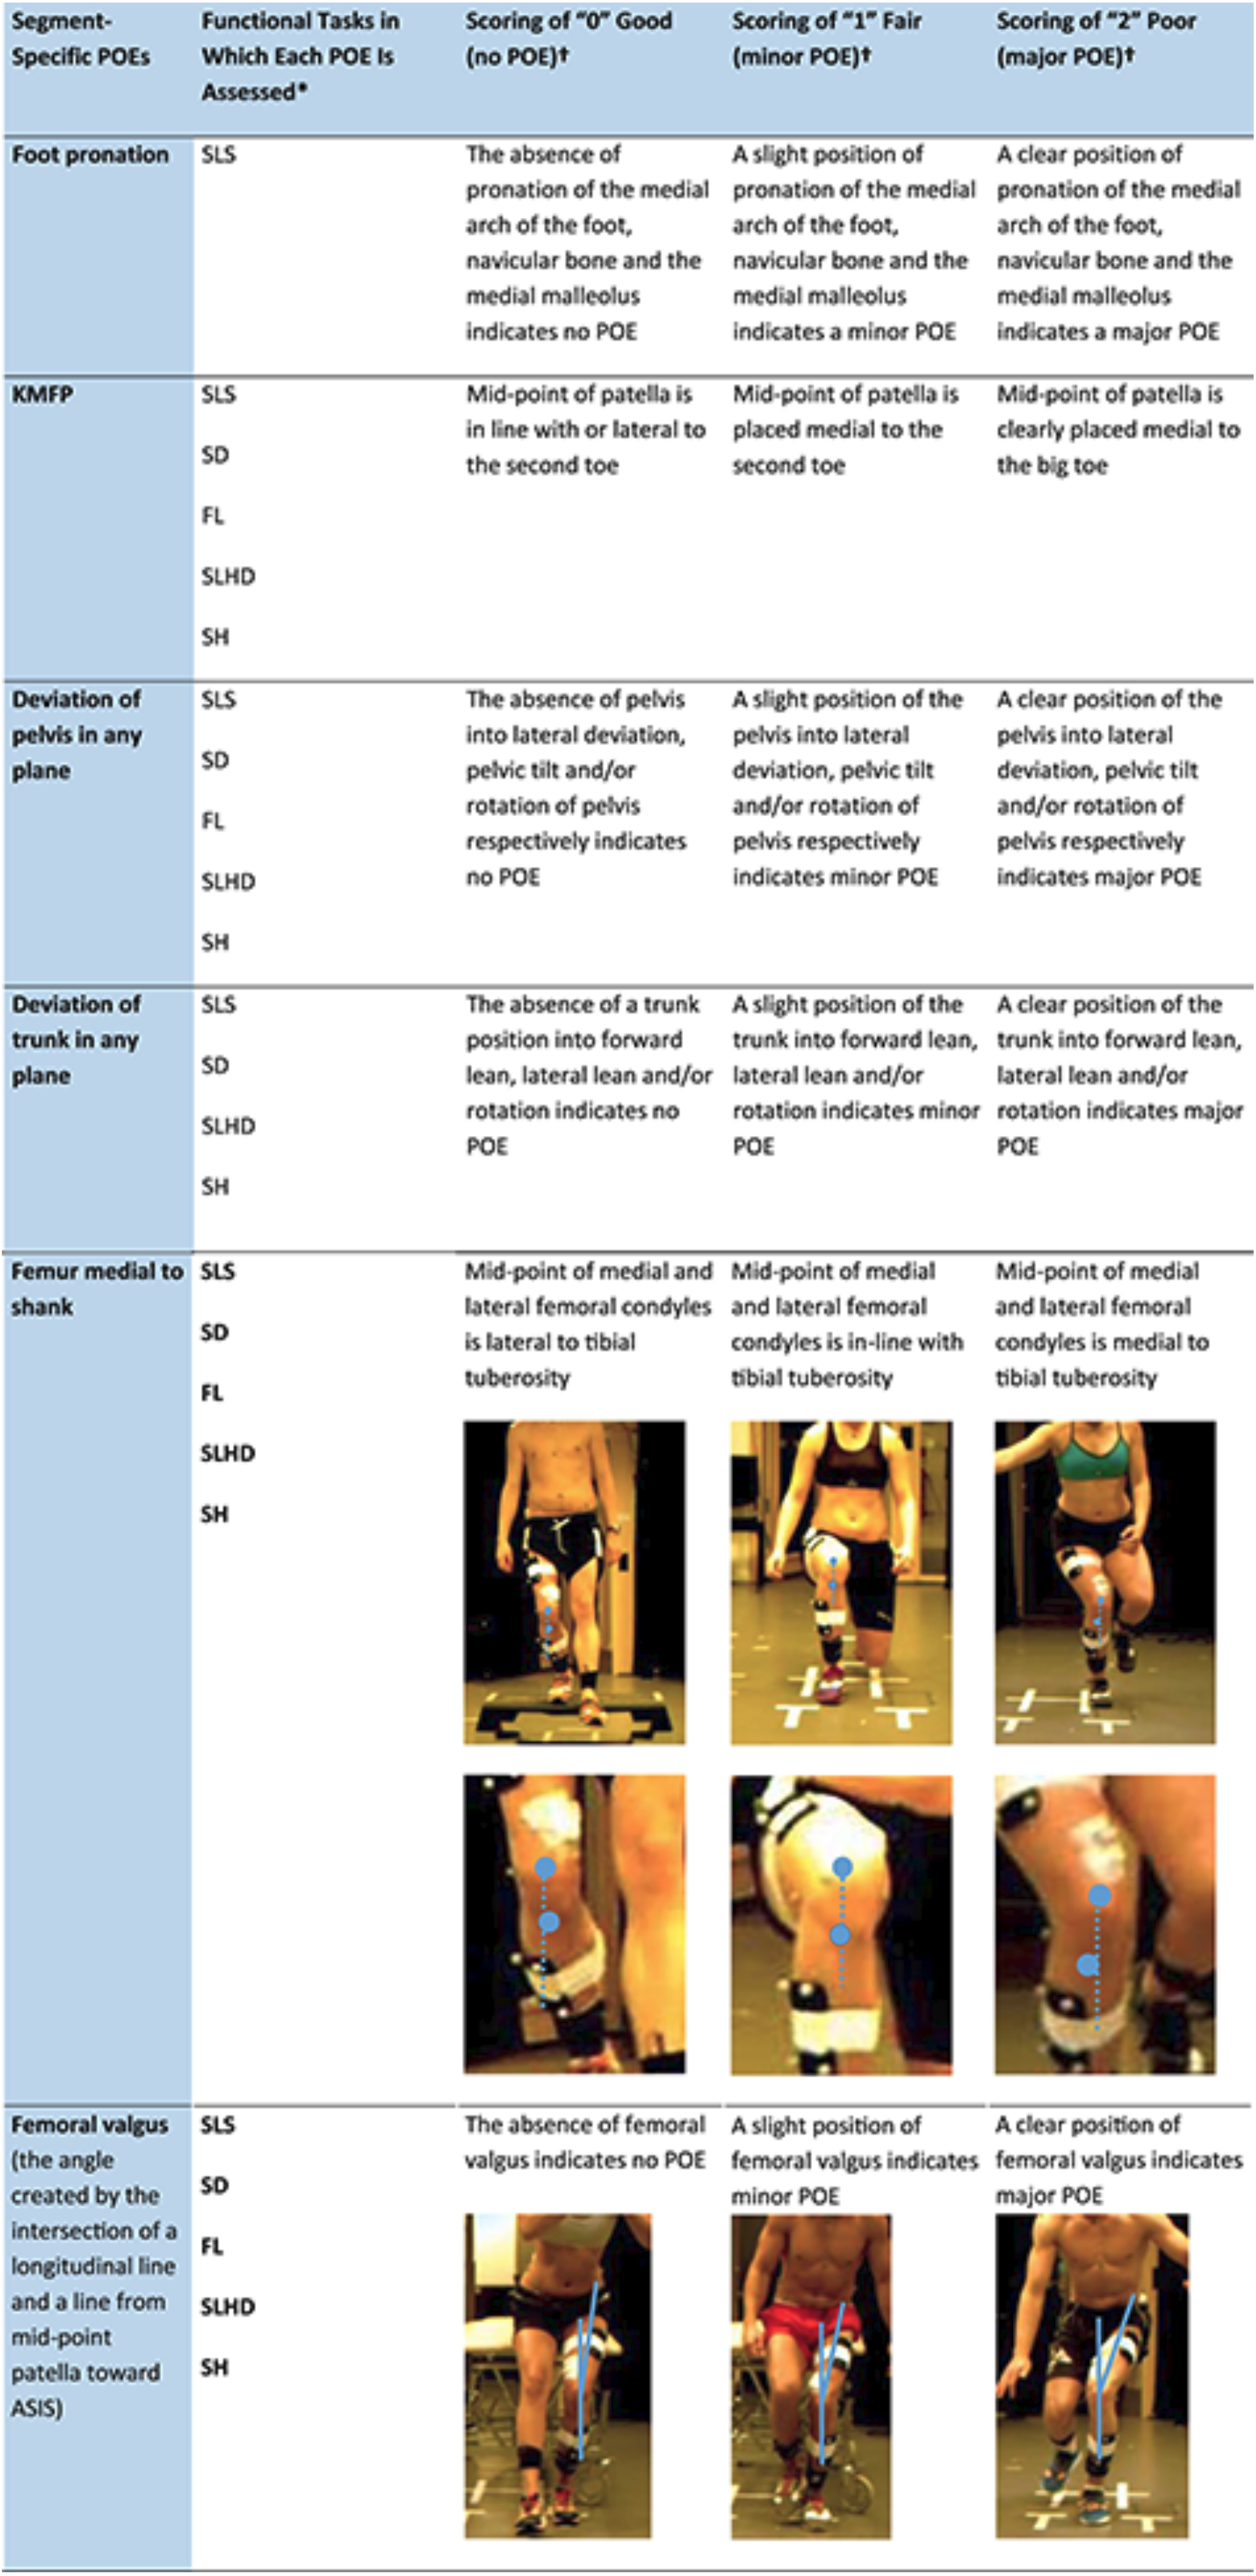
\includegraphics[height=\textheight]{files/figs/poes-detailed-rot.png}
  % \caption{}
  \label{}
\end{figure}


\chapter{wtf}
this is the information

\newpage
% This is the last page of the document
\thispagestyle{empty}
\AddToShipoutPictureBG*{%]
    \AtPageLowerLeft{%
        
\includegraphics[width=1.0\paperwidth]{setup/img/kth-footer.png}
    }%
}

\PlaceText{20mm}{282mm}{\color{white}\fontsize{12}{0}\sffamily www.kth.se }


\end{document}
